% \documentclass[a4paper]{article}
\documentclass[12pt]{extarticle}
\usepackage[a4paper, left=1.5cm, right=1.5cm, top=1.5cm, bottom=2.0cm]{geometry}
\usepackage{graphicx} % Required for inserting images
\usepackage{caption}  % for continuedfloat

\usepackage{lscape} % For landscape pages
\usepackage{afterpage}
\usepackage{pdflscape} % To create landscape pages that show as landscape in PDF viewer
\usepackage{parskip} % Adds white space between paragraphs
\usepackage{amsmath}

\bibliographystyle{plain} % We choose the "plain" reference style

\title{Chance of stroke from population demographics}
\author{Anna Laws}
\date{August 2025}
\begin{document}

\maketitle



\section{Introduction}

% %%%%% Concept of need to predict admissions using stuff we always know (ideas of usage) %%%%%
As England’s population grows and ages in the coming decades \cite{projections_2025}, it will be increasingly important to ensure that emergency stroke units are properly resourced. By combining reliable forecasts of population demographics with the average stroke risk of comparable groups, it should be possible to estimate future stroke incidence more accurately.


% %%%%% Intuition that admissions should depend on age and deprivation %%%%%
Intuitively the main predictive factors for stroke should be specific signs of poor health where the data are incomplete and unavailable on large scales,
so instead we seek available data that indicate poor health.
% 
We expect that poorer health is more likely, and so stroke admissions typically higher, in people of higher age and/or living in higher levels of deprivation as measured by the Index of Multiple Deprivation, which includes factors such as access to healthcare, education, and earnings. 


% %%%%% What we've actually found %%%%%
% Generic groups:
We model the number of strokes in a group of people as the product of its number of people $n_{\textnormal{group}}$ and the probability of its members having a stroke, $P(\textnormal{stroke} | \textnormal{group})$.
% Age/depriv groups:
We define 25 groups, one for each combination of five age bands and five deprivation levels.
The age bands are defined as people under 65, aged 65--69, aged 70--74, aged 75--79, and 80 and over,
both to pick out the detailed changes in stroke incidence at older ages from the population of today, 
and because the relative numbers of people in these bands in England are expected to increase over the next twenty years due to the post-war baby boom.
The five deprivation levels are defined as quantiles, i.e. each group contains 20\% of the English population from most-deprived to least-deprived areas,
where five groups are expected to be sufficient to detect a difference and too few to be confounded by other factors such as geography.
% 
The resulting total number of strokes strokes across England $a$ is then
$a = \sum P(\textnormal{stroke} | \textnormal{age, deprivation}) \cdot n_{\textnormal{age, deprivation}}$.
% 
Once the coefficients $P$ have been quantified then the number of strokes can be calculated for any population with a known breakdown by age band and by regional deprivation levels comparable with those in England. %, including areas outside England and with projected demographics in the future.


% %%%%% Method overview %%%%%
We calculate values for the coefficients $P$ using national-level and MSOA-level stroke admissions and population demographic data.
%
At the MSOA level, the number of all recorded strokes in England averaged across 2017 to 2019 inclusive is available from Hospital Episode Statistics (HES),
and the deprivation ranking Index of Multiple Deprivation (IMD) and the number of people in each age band in mid-2020 from the Office for National Statistics (ONS).
Nationally, the number of admissions to emergency stroke units in England from people in each age band for the same date range as the HES data is taken from the Sentinel Stroke National Audit Programme (SSNAP),
and the number of people in each age band in January 2019 from the ONS.
% 
There is no data available that provides stroke incidence by age band and by deprivation level simultaneously,
so we use the national-level data to find the pattern of stroke incidence with age,
and then factor in deprivation level using the MSOA-level data.

The aim is to find a set of age-deprivation coefficients $P(\textnormal{stroke} | \textnormal{age, deprivation})$ that produces the most accurate numbers of strokes for all MSOA simultaneously rather than seeking perfect accuracy for each MSOA
because the MSOA-level observed stroke numbers contain random errors.
These data cover only three years and so by chance some MSOA will have recorded far more or far less than than the true average,
and the difference of one stroke is substantial for typically around 10 annual strokes per MSOA.
%
In this document,
we examine the available data to confirm the intuition that stroke admissions increase with age and with deprivation.
Then we use national data to calculate values of the coefficients $P(\textnormal{stroke} | \textnormal{age})$.
We test many variations of the age-derived coefficients using a genetic algorithm,
the best results of which are then refined by searching the parameter space immediately adjacent to those coefficients.
% 
The resulting derived coefficients are applied to the catchment areas of emergency stroke units in Devon and Cornwall to illustrate the potential change in admission numbers up to 2040.


\section{Defining age-deprivation coefficients}

\begin{figure}
    \centering
    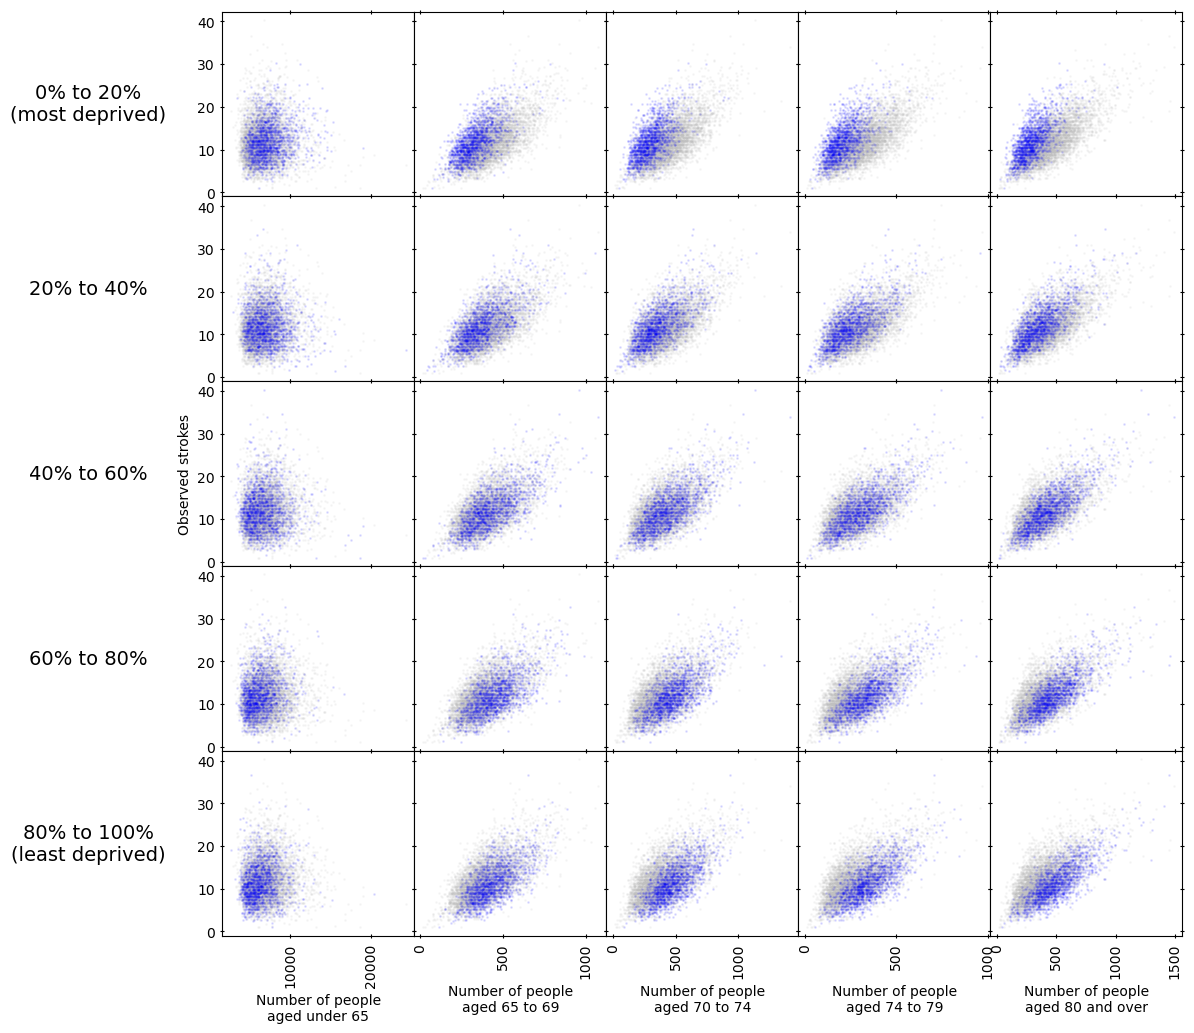
\includegraphics[width=1.0\linewidth]{images/scatter_age_admissions_by_imd.png}
    \caption{
    Comparison of the numbers of people in each age band with the number of admissions for each MSOA, split by deprivation level. The grey markers show data for all MSOA in all cases and coloured markers show the data for only MSOA in the stated deprivation level.
    Note: the admissions are the total from all age bands, not just the age band relevant to each panel.
    }
    \label{fig:scatter_age_admissions_by_imd}
\end{figure}

% \begin{table}
% \centering
% \caption{Percentage of population in each age band by deprivation level.}
%     \begin{tabular}{lrrrrr}
%         Proportion with age: & $<$65 & 65--69 & 70--74 & 75--79 & 80+ \\
%         \hline
%         % Deprivation quantile &  &  &  &  &  \\
%         0-20\% (most deprived) & 86.0 & 4.1 & 3.7 & 2.6 & 3.6 \\
%         20-40\% & 83.2 & 4.6 & 4.5 & 3.2 & 4.5 \\
%         40-60\% & 79.7 & 5.4 & 5.5 & 3.9 & 5.5 \\
%         60-80\% & 77.7 & 5.7 & 6.1 & 4.4 & 6.1 \\
%         80-100\% (least deprived) & 77.6 & 5.6 & 6.0 & 4.4 & 6.4 \\
%     \end{tabular}
%     \label{tab:demogs_by_depriv}
% \end{table}

Initially we check for relations between admissions and demographic variables in the MSOA-level data.
% 
The number of people in the older age bands (age over 65) and the admissions numbers have a good correlation that becomes stronger when the MSOA are split by deprivation quantile.
% 
Figure~\ref{fig:scatter_age_admissions_by_imd} shows that
% the data for the most deprived quantiles (top row) tend to appear further left and higher up than the least deprived quantiles (bottom row).
% This means that 
to reach the same number of stroke admissions, fewer people are needed in the older age groups in more deprived areas than in the less deprived areas. In other words, the probability of stroke is higher with age in more deprived areas.
% 
% %%%%% STROKE PROB INCREASES WITH DEPRIVATION %%%%%
All five deprivation quantiles have roughly the same population by definition, and the proportion of people aged 65 and over in the most-deprived quantile is 71\% of the proportion in the middle quantile.
If the stroke admissions were mostly being driven by the people aged over 65 and had no effect from deprivation,
then the admissions in the most-deprived quantile should be around 71\% of those of the middle quartile.
However the total stroke admissions from most to least deprived levels are 16420, 16204, 16442, 16419, and 15473,
suggesting that stroke incidence increases with deprivation level for all age bands.


% %%%%% CALCULATE SSNAP COEFFS %%%%%
% \clearpage  % force first figure to show before this table is drawn
\begin{table}
\centering
    \caption{Stroke coefficients from SSNAP data. England population is 56.3 million in January 2019 and total annual strokes are 80,958.}
    \begin{tabular}{crrr}
    Age Groups & Percentage of all population & Annual admissions & $P(\textnormal{stroke} | \textnormal{age})$ \\% Probability of stroke given age \\
    \hline
    Less than 65 & 81.6\,\% & 18737.7 & 0.04\,\% \\
    65--69 & 5.0\,\% & 7395.3 & 0.26\,\% \\
    70--74 & 5.0\,\% & 10379.6 & 0.37\,\% \\
    75--79 & 3.4\,\% & 11654.6 & 0.60\,\% \\
    80+ & 5.0\,\% & 32790.8 & 1.16\,\% \\
    \end{tabular}
    \label{tab:ssnap_coeffs}
\end{table}

\begin{figure}
    \centering
    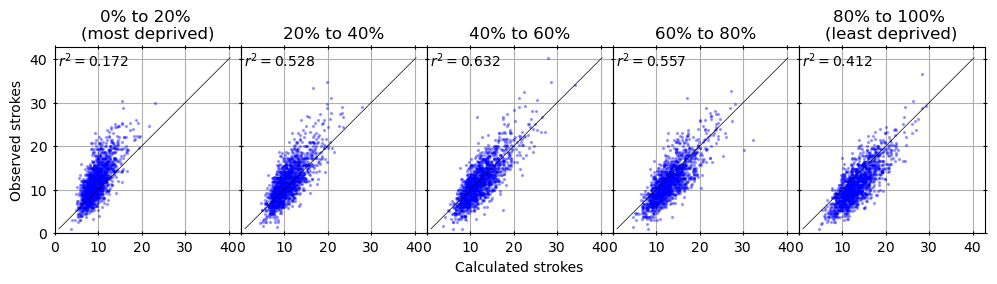
\includegraphics[width=1.0\linewidth]{images/scatter_admissions_from_ssnap_coeffs_separate_1row.png}
    \caption{Comparison of the numbers of admissions calculated using the age-band-derived coefficients with the observed admissions in each MSOA, split by deprivation level. The black diagonal line marks where the two measures are equal.}
    \label{fig:scatter_admissions_from_ssnap_coeffs_separate}
\end{figure}

We can calculate probabilities of stroke given only age band, $P(\textnormal{stroke} | \textnormal{age})$, by combining national population demographics with national stroke incidence data.
To calculate national annual numbers of stroke by age band, take the mean national emergency admissions across the available years and scale up the results by 1.45, which is the ratio of the total annual admissions for all stroke and for only emergency stroke admissions.
% 
The ratio of the resulting numbers of stroke to the England population data gives the probability of stroke given a certain age band shown in Table~\ref{tab:ssnap_coeffs}.
% 
% %%%%% SSNAP COEFFS RESULTS %%%%%
We test these coefficients by calculating the annual numbers of stroke from each MSOA and find the R-squared value of the calculated to observed admissions is 0.46. 
% 
Figure~\ref{fig:scatter_admissions_from_ssnap_coeffs_separate} is a scatter plot of the observed and calculated numbers of stroke for all MSOA in each deprivation quantile, and shows that admission numbers are largely under-predicted for the most-deprived MSOAs and over-predicted for the least-deprived MSOAs.
% 
Therefore a better predictor of annual numbers of strokes at the MSOA level should be found
by allowing different coefficients for each deprivation group.



% %%%%% FITNESS %%%%%
The quality of a set of age-deprivation coefficients is judged by combining two accuracy measures. 
These are the sum of square residuals between predicted and observed numbers of stroke across all English MSOA, and
a ratio derived from the national-level strokes in each age band.
An error ratio is defined for each age band as the absolute difference between 1 and the ratio of predicted to observed strokes, 
$|1 - \frac{\textnormal{predicted admissions}}{\textnormal{observed admissions}} |$,
and the five error ratios are summed into a single value.
The two accuracy measures are multiplied together to create a measure of fitness, where the main contribution is from the MSOA-level accuracy with a modification factor from the age band accuracy.
% The error ratio prevents the case where one age band has many more and another age band many fewer national admissions than observed in the SSNAP data so that the total amount is close to correct, but the individual age bands are inaccurate.


\section{Optimisation}
% %%%%% SEARCH MANY OPTIONS %%%%%
We can find the age-deprivation coefficients $P(\textnormal{stroke} | \textnormal{age, deprivation})$ by using two stages of optimisation:
a genetic algorithm to explore a large number of combinations of coefficients;
and a nudge method to check the parameter space immediately around the best sets of parameters.

% %%%%% STARTING COEFFICIENTS %%%%%
We ensure each set of age-deprivation coefficients is on the right order of magnitude by building it from five copies of the age-derived coefficients in Table~\ref{tab:ssnap_coeffs} that are scaled up or down by a small factor.
The scale factors are in steps of 0.1 in the range 0.2 to 2.0, which was selected because no test cases outside this range provided good accuracy.
% 
We only keep the 2659 combinations that are more likely to have good accuracy because the following conditions are met:
the scale factor must remain constant or increase for more-deprived quantiles;
the sum of scales must be between 4 and 6 inclusive to prevent cases where all scale factors are either large or small;
no more than three scale factors may be 1 or higher;
and no more than three scale factors may be 1 or lower. 
% The first and final two conditions combined force the middle scale factor to always have a value of 1.
Next the fitness of the 25 age-deprivation coefficients derived from each set of scale factors is checked.
The best set has a fitness of 253.2, and we keep only the 886 sets of factors with fitness no more than twice this best fitness value.


% %%%%% GENETIC ALGORITHM SUMMARY %%%%%
We search the parameter space around the 886 starting sets of coefficients using a genetic algorithm. With this method we compare many sets of coefficients, select the best, and combine sets to create brand-new sets. This allows us to explore as much parameter space (try as many combinations of coefficients) as is reasonable.
% 
In each generation of the algorithm, sets of coefficients are paired up and given a chance of crossover, where a random series of their coefficients are swapped over. Then each set of coefficients has a chance of mutation, where some of its coefficients are adjusted slightly at random, for example from a scale factor of 1.4 to 1.32. The algorithm uses high mutation and crossover rates to sample as much variation in the coefficient values as possible.
Any sets of coefficients that are generated are adjusted if necessary so that the coefficients always increase or remain constant with increasing age band or deprivation level.
Then a set of individuals are picked out to continue to the next generation with preference given to sets of coefficients with better fitness scores.

% %%%%% RUNNING DEAP %%%%%
We use DEAP \cite{DEAP_JMLR2012} to create the genetic algorithm.
The genetic algorithm starts with 300 individuals picked from the 886 options. 
Each individual is defined as a set of of 25 scale factors because these are the same order of magnitude and so can be mutated with the same parameters.
An individual has a 95\% chance of mutation, but each of its scale factors has only a 4\% chance of mutating so that on average only one of its values change. Scale factors are mutated by adding on a factor sampled from a Gaussian distribution with a mean of 0 and standard deviation of 0.1.
The 300 individuals are assigned into 150 pairs where each pair has an 80\% chance of two-point crossover, where the start and end points of the crossover are selected at random. The 25 scale factors are ordered by starting with the highest deprivation, listing the five age bands, then moving to the next-most-deprived, listing the five age bands, and so on until all 25 groups have been placed in the order. This means that the two-point crossover will be more likely to affect multiple age bands in the same deprivation level and less likely to cover multiple deprivation levels.
Finally, the best individuals are selected for the next generation using a tournament. For each of the 300 places in the next generation, three individuals from the current generation are picked at random. Of these three, the individual with the best fitness is chosen for the next generation. 
% 
We run the simulation 100 times with different random selections of starting individuals.
Each simulation continues until either 1000 generations have passed or all of the individuals have similar coefficients (standard deviation is less than 5\% of the mean for each coefficient). When all individuals are so similar, there is not much further improvement to be gained from crossover.
We keep a copy of the best individual from each generation of each of the 100 simulations.
The 100 best sets of coefficients use the best individual seen in any generation of each run.


% %%%%% GENETIC ALGORITHM RESULTS %%%%%

\begin{figure}
    \centering
    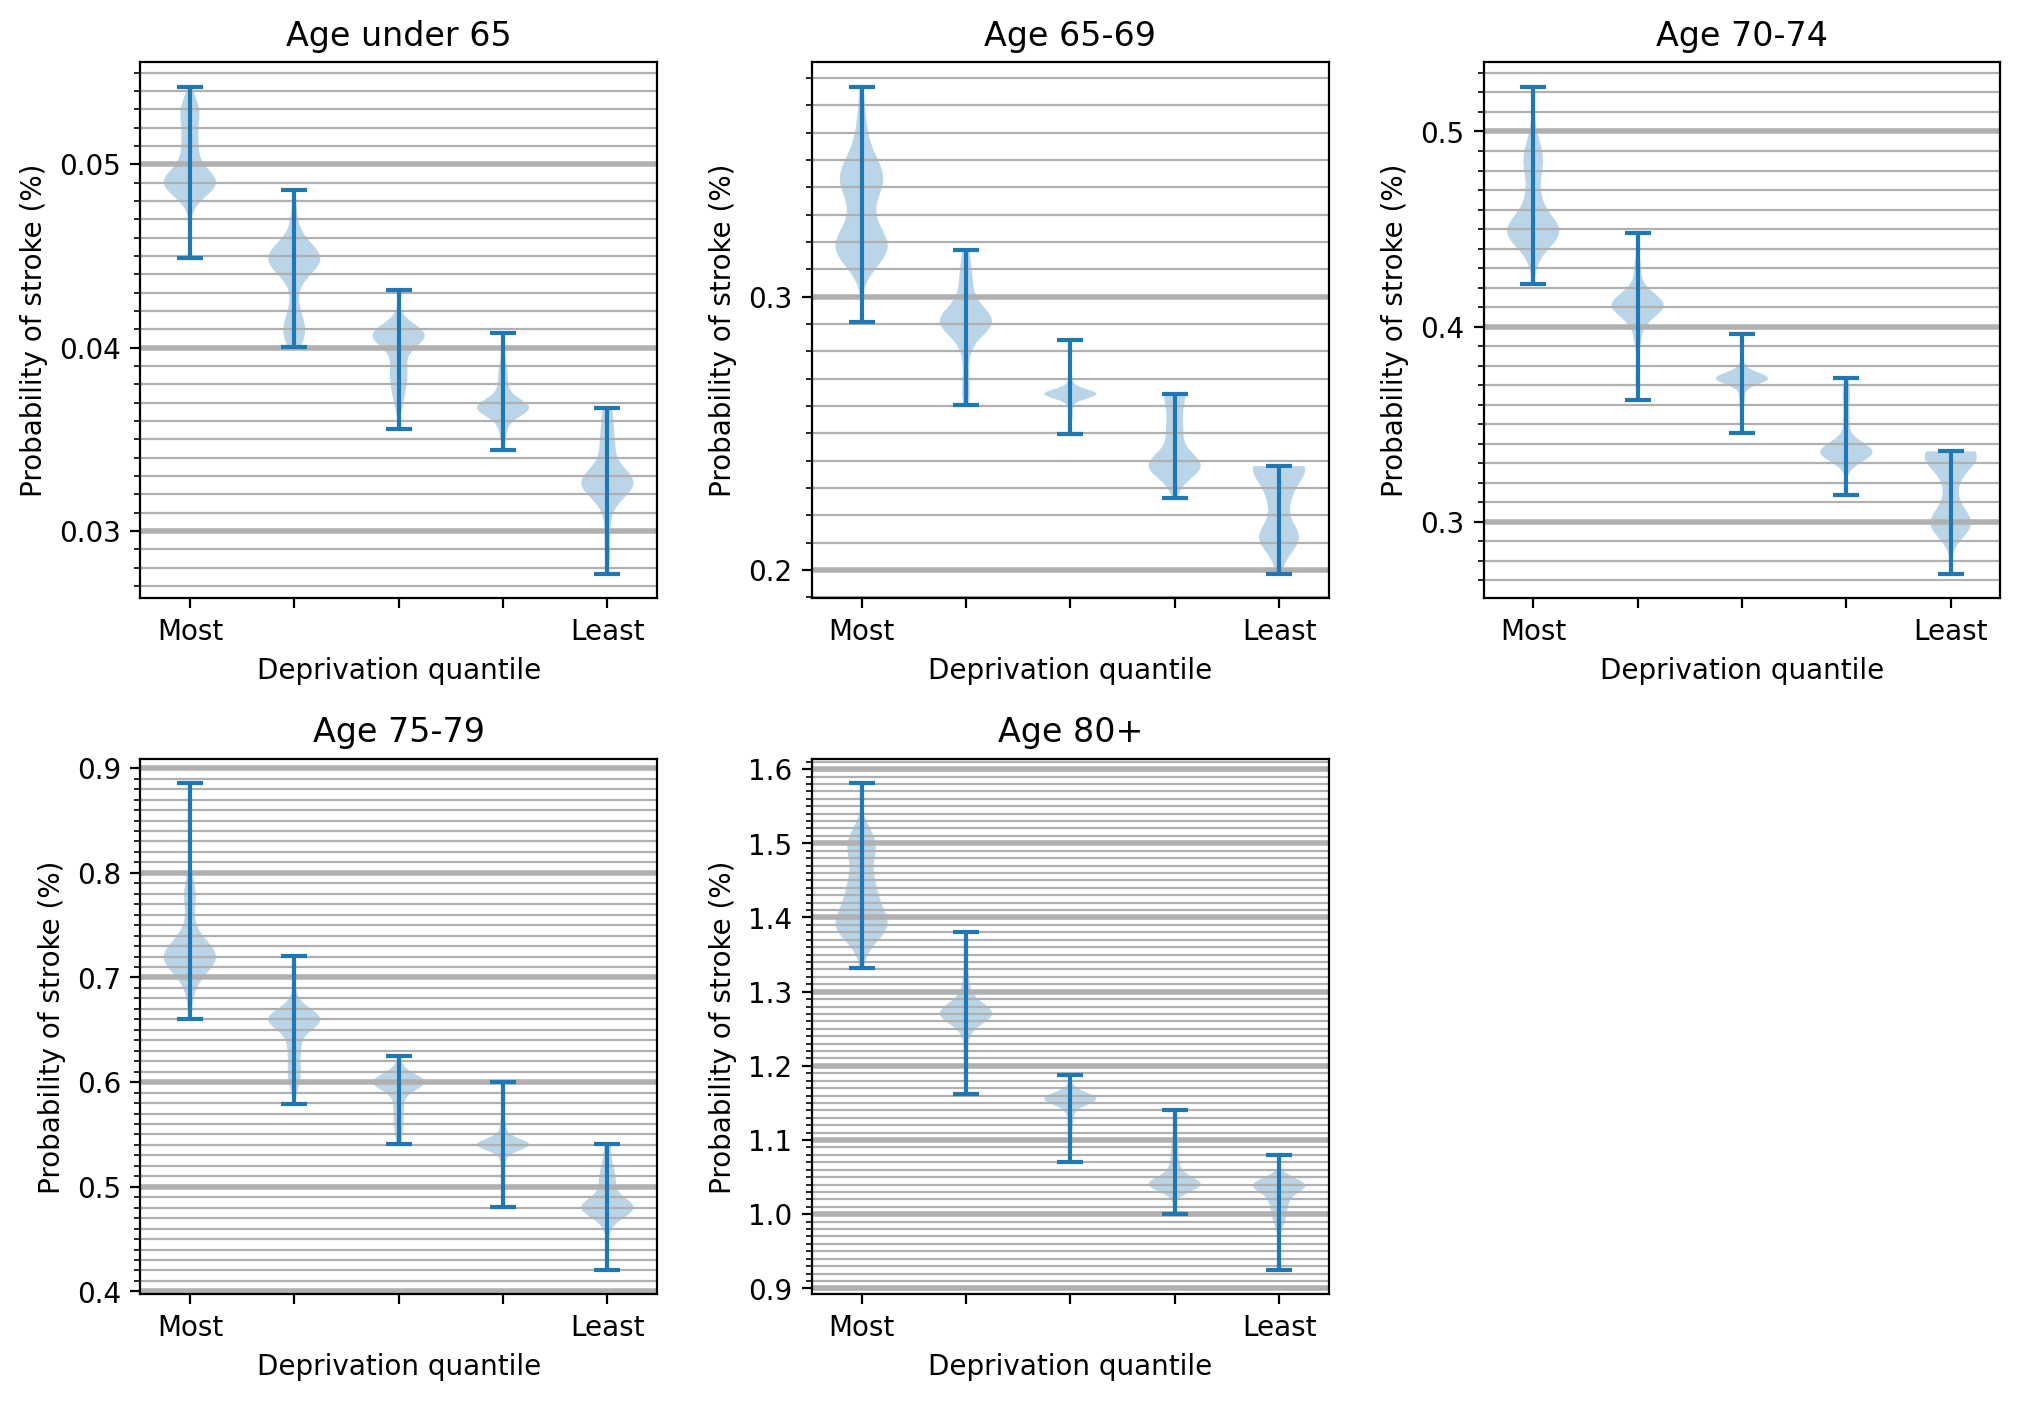
\includegraphics[width=1.0\linewidth]{images/violin_coeffs_deap_output.png}
    \caption{Violin plots of the 100 sets of coefficients found from the genetic algorithm.}
    \label{fig:violin_coeffs_from_deap}
\end{figure}

The 100 best sets of coefficients have similarly-good fitness scores ranging from 237.7 to 240.6 and no convergence onto a similar set of values, even when rounded to only one significant figure, although the resulting numbers of stroke are similar.
The variation in coefficients can be seen in the violin plots of Figure~\ref{fig:violin_coeffs_from_deap}.
% 
For each MSOA, the 100 sets of predicted strokes can be compared to find a separate standard deviation. Then the mean of these 6790 standard deviations is 0.164 % or only 1.4\% of the predicted admissions.
and the average predicted strokes across all MSOA is 11.9.
An area containing 70 such average MSOA would have 834.8 strokes with a standard deviation of only 1.4 strokes across the 100 sets of coefficients. 
% 
It would be difficult to search the huge parameter space for a global minimum (true best answer) of a single set of coefficients at a high precision,
and there is no expectation that it would give large gains in fitness.
% Instead we drop the precision of the age-deprivation coefficients to fewer significant figures.
Instead we round the age-deprivation coefficients to 2 significant figures (s.f.) for the age 80+ group and 1 s.f. for the rest.
The over-80 age band uses an extra significant figure because the values of all its coefficients from the genetic algorithm output lie between 0.009 and 0.016, so only one significant figure is not enough to show any variation across deprivation.
This balances the worsening of attainable fitness with an understanding that fewer sets of coefficients will have similarly good levels of fitness,
meaning that the final result will be more trustworthy as the best possible at that precision.


% %%%%% NUDGE WALK %%%%%
We can robustly search the parameter space near a set of 25 coefficients by tweaking the coefficient values to find any better combinations.
This is more reasonable when the coefficients have been rounded to fewer significant figures since the number of possibilities is reduced from infinite to a large but feasible number.
% When the other age bands use 2 significant figures, we ran both 2 and 3 figures for the over-80 age band in case 2 was still not enough to see any variation as most values lie well within one step with 2 s.f.
% 
We consider a ``nudge'' as an increase or decrease of one step of precision equal to the precision of the number.
%, for example a coefficient 4e-3 may change to 3e-3 or 5e-3 with one nudge and a coefficient 1.3e-2 may change to 1.2e-2 or 1.4e-2.
% 
Then we define a reasonable variation on a set of coefficients as: one coefficient increases or decreases by 1 nudge or by 2 nudges; or one coefficient increases by 1 nudge or 2 nudges and another decreases by 1 nudge or 2 nudges.
The pairs of coefficients that change together must share either an age band or a deprivation level.
% 
Pairing the coefficients in this way makes it likely that the total national numbers of stroke will see little change and some strokes can be shifted from one age-deprivation group into another to improve the discrete age-band accuracy or deprivation-level accuracy.
There are a total of 900 possible nudge combinations from 25 coefficients, with 4 sets of 25 options where 1 coefficient changes and 4 sets of 200 options where 2 coefficients change.
% 
For a starting set of coefficients, the 900 sets of nudged coefficients are found and any sets that do not increase with age band or with deprivation are discarded.
The remaining set with the best fitness is selected and used as the basis for the next set of 900 nudges.
This process is repeated until the same best set has been selected twice, meaning that no better coefficients are available.
% 
The final derived coefficients cannot be improved by any of the possible 900 nudges and so a local minimum has been found for this discrete parameter space.


\section{Results}


\begin{table}
\centering
\caption{Final coefficients for $P(\textnormal{stroke} | \textnormal{age, deprivation})$ (\%).}
    \begin{tabular}{l l l l l l}
    Deprivation / age group & $<65$ & 65--69 & 70--74 & 75--79 & 80+ \\
    \hline
    0-20\,\% (most deprived) & 0.06 & 0.5 & 0.5 & 0.7 & 1.2 \\
    20-40\,\% & 0.05 & 0.3 & 0.4 & 0.7 & 1.2 \\
    40-60\,\% & 0.03 & 0.2 & 0.4 & 0.6 & 1.2 \\
    60-80\,\% & 0.03 & 0.2 & 0.4 & 0.5 & 1.1 \\
    80-100\,\% (least deprived) & 0.03 & 0.2 & 0.2 & 0.5 & 1.1 \\
    \end{tabular}
    \label{tab:final_coeffs}
\end{table}



% %%%%% UNCERTAINTY %%%%%

\begin{figure}
    \centering
    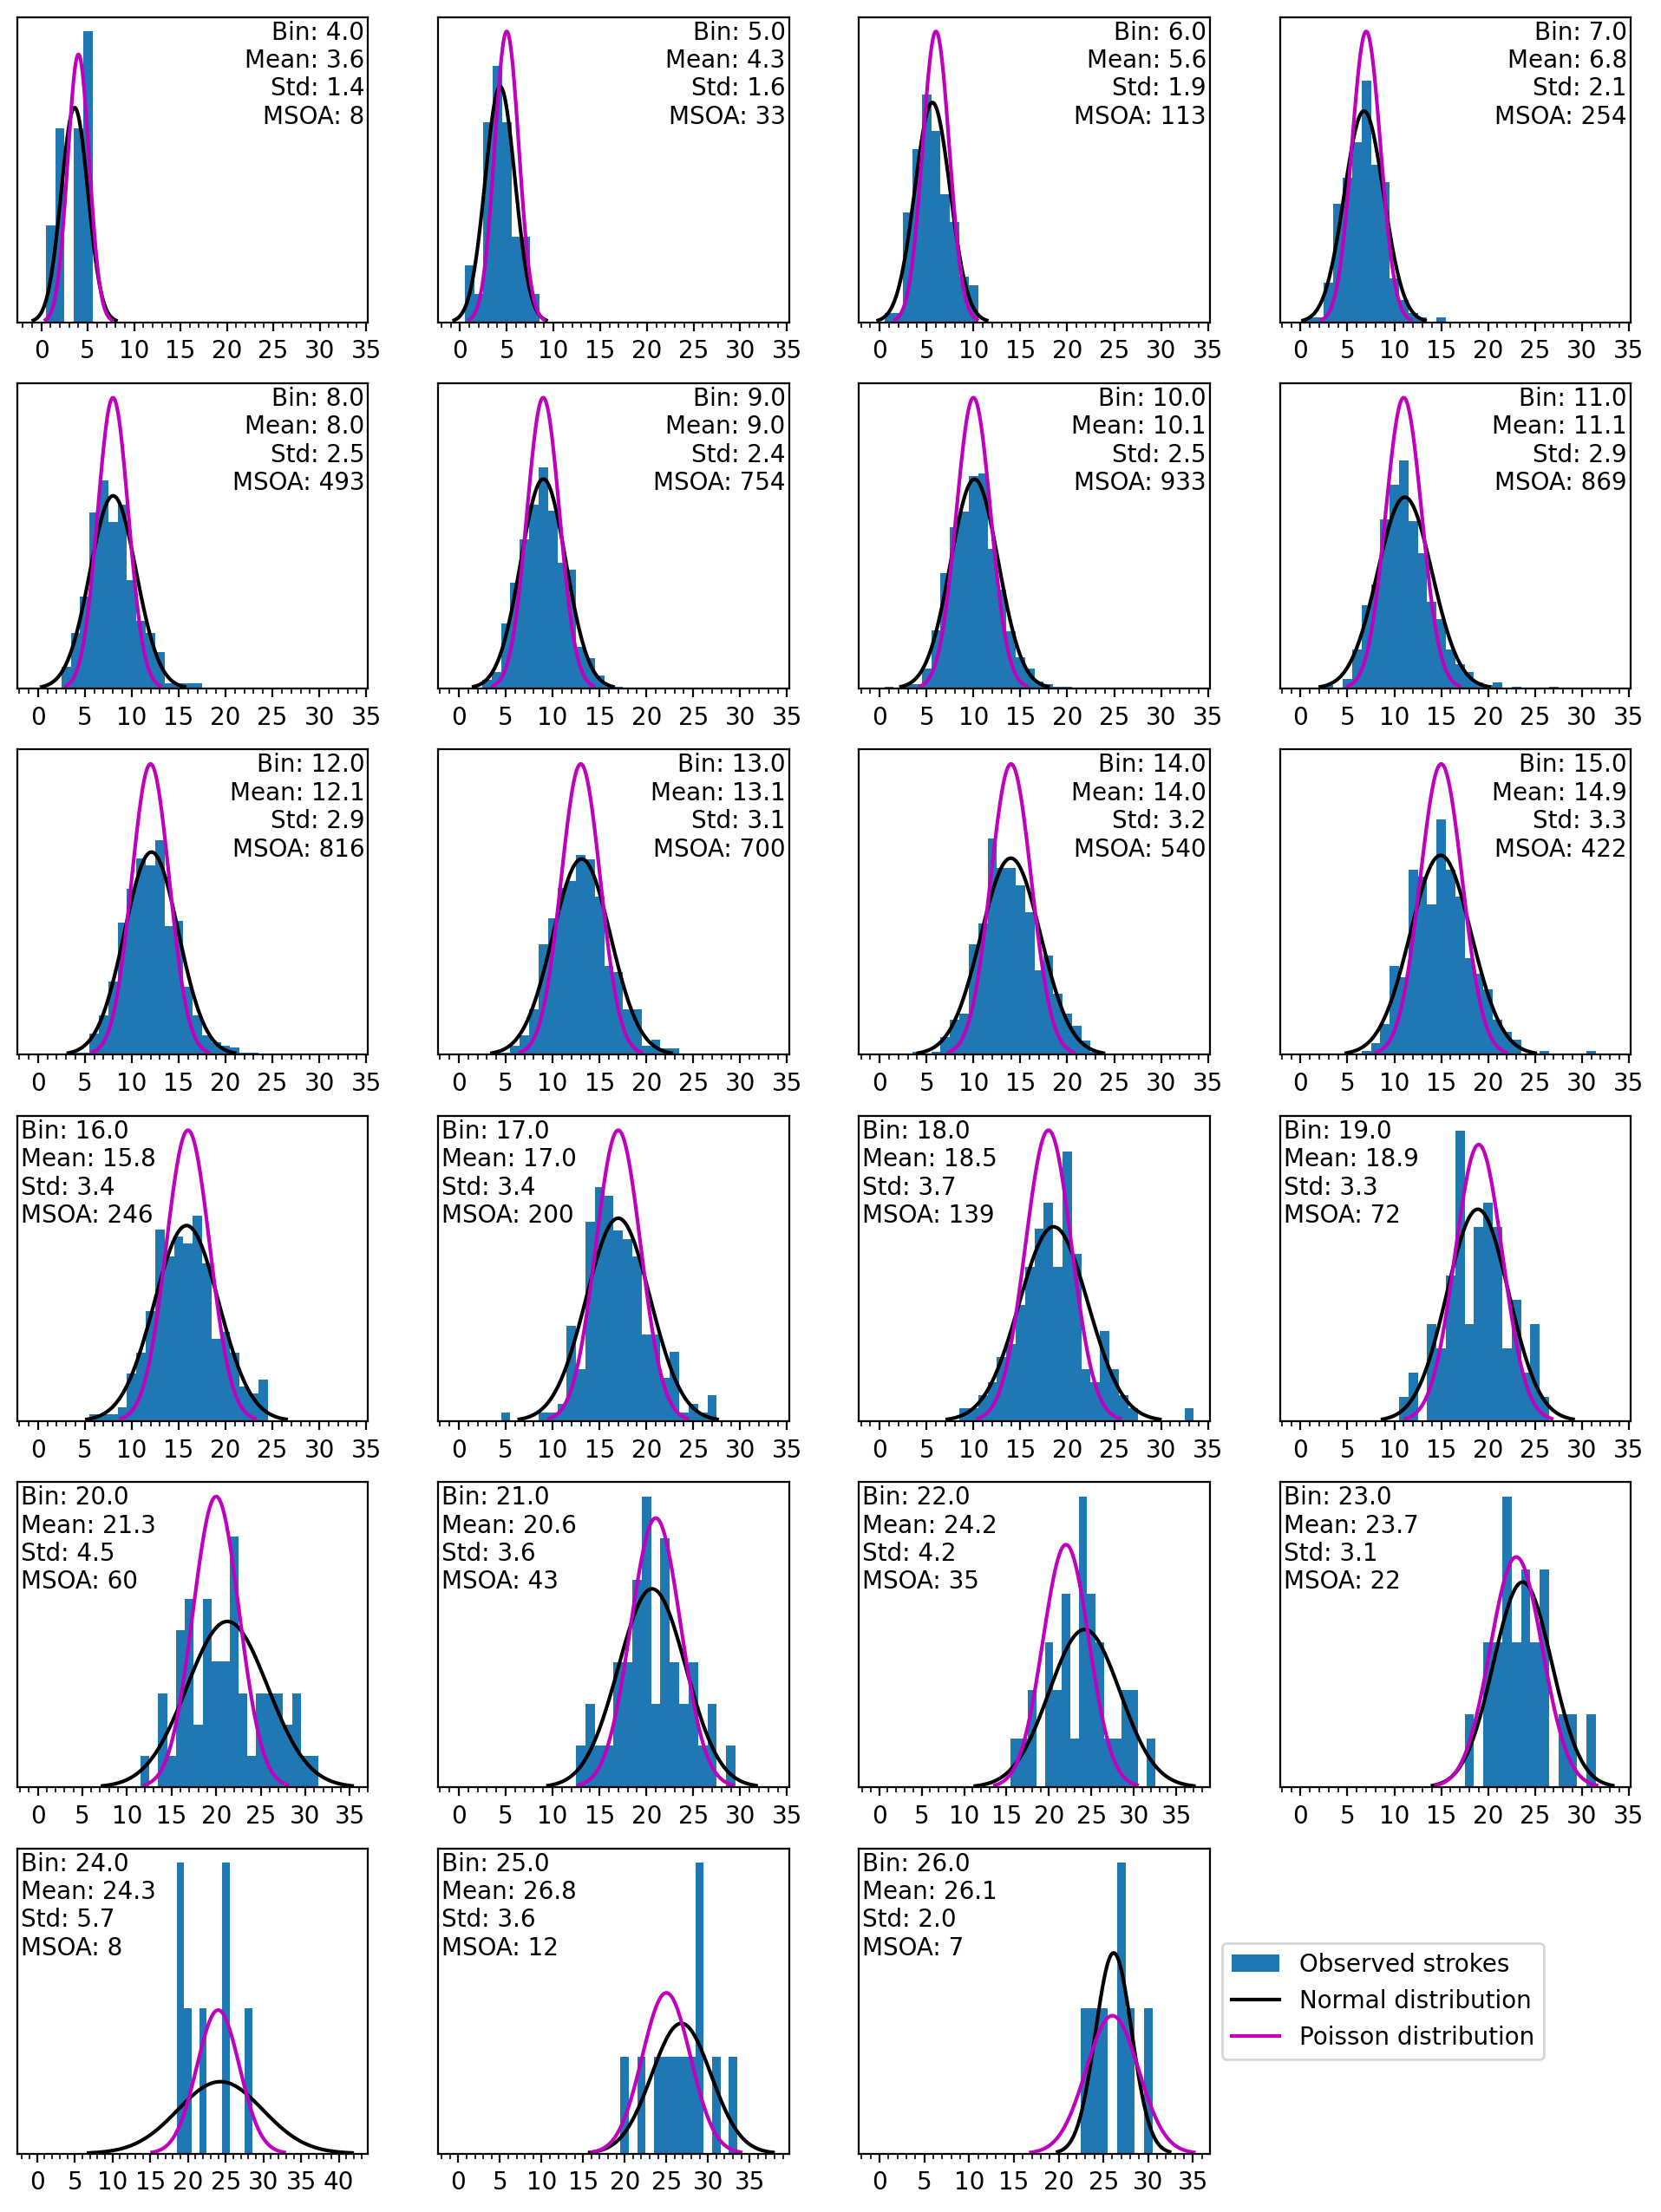
\includegraphics[width=1.0\linewidth]{images/uncertainty_observed_admissions_variance.png}
    \caption{
        Histograms of the observed numbers of strokes in each bin of predicted strokes. 
        The normal distribution uses the same mean and standard deviation as the observed stroke data,
        and the Poisson distribution uses the variance expected from the predicted stroke number for the mean of three samples.
        }
    \label{fig:uncertainty_hists}
\end{figure}

\begin{figure}
    \centering
    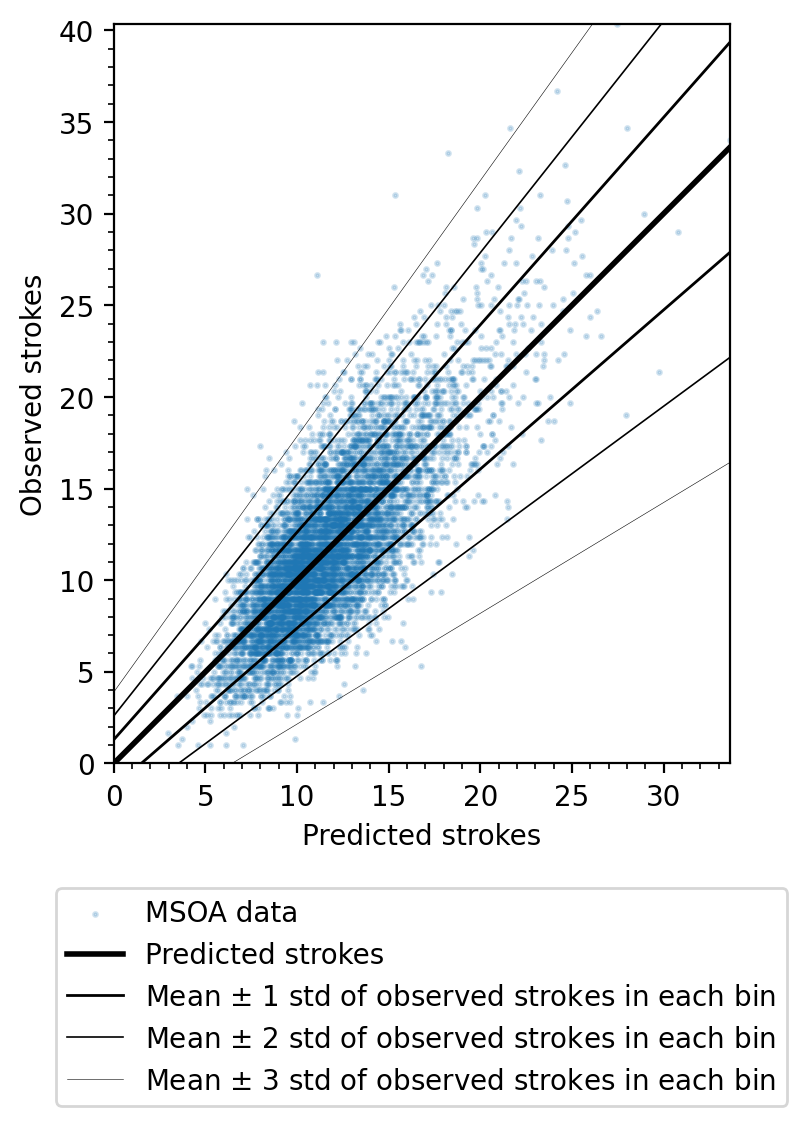
\includegraphics[width=0.5\linewidth]{images/uncertainty_fitted_std.png}
    \caption{Scatter of predicted and observed numbers of stroke with line fits to standard deviation of predicted strokes.}
    \label{fig:uncertainty_fitted_std}
\end{figure}


This method was applied to the 100 sets of coefficients from the genetic algorithm output. 
The resulting best set of age-deprivation stroke coefficients in Table~\ref{tab:final_coeffs} has fitness 244.2 and was found by 21 separate starting sets of coefficients.

The final age-deprivation coefficients were used to predict the number of strokes for each of the English MSOAs.
% 
To find a measure of the precision of the predicted values, the MSOAs were grouped by their nearest whole number of predicted strokes. Figure~\ref{fig:uncertainty_hists} shows that the distribution of the observed strokes in each group resembles a normal distribution with its central value and spread matching the mean and standard deviation of the observed strokes, with the best matches for groups that contain at least 200 MSOAs (whole number of predicted strokes between 7 and 17 inclusive).
% 
For these groups, the standard deviation of observed strokes increases as the predicted strokes bin increases.
%
A linear regression was fitted to the means $\mu$ and standard deviations $\sigma$ of these groups (data printed in annotations of Figure~\ref{fig:uncertainty_hists}) to find $\sigma = 0.13\mu + 1.30$ within those bounds (R-squared 0.95).
This fit is overlaid on the scattered predicted and observed numbers of strokes in Figure~\ref{fig:uncertainty_fitted_std}, which shows that most of the observed values lie within one or two standard deviations of their predicted value.
% 
A realistic predicted number of strokes can therefore be found using random samples of a normal distribution with the mean and standard deviation respectively of the strokes predicted from the age-deprivation coefficients and the formula for standard deviation $\sigma$.



\begin{figure}
    \centering
    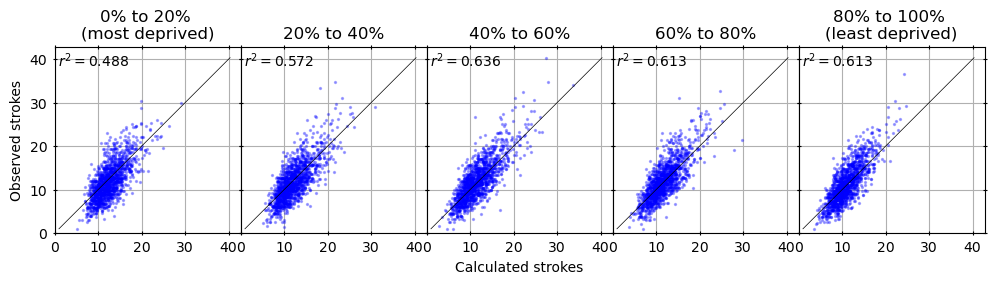
\includegraphics[width=1.0\linewidth]{images/admissions_prediction_comparison_separate_1row.png}
    \caption{Comparison of the numbers of strokes calculated using the deprivation-derived coefficients with the observed values in each MSOA, split by deprivation level. The black diagonal line marks where the two measures are equal.}
    \label{fig:admissions_prediction_comparison_separate}
\end{figure}


% %%%%% R-SQUARED %%%%%
Figure~\ref{fig:admissions_prediction_comparison_separate} shows the strokes for all MSOA from the age-deprivation coefficients split into separate panels for each deprivation quantile, and has is less variation from the equality diagonal line than for the age-only coefficients in Figure~\ref{fig:scatter_admissions_from_ssnap_coeffs_separate}.
While previously there was a noticeably worse fit for the most-deprived areas (R-squared 0.01), this effect has reduced when using the final coefficients (R-squared 0.49), and the overall R-squared values have also increased from 0.46 to 0.59.

% %%%%% APPLY WRONG DEPRIVATION COEFFS %%%%%
As a further test of the derived coefficients, we can compare the predicted strokes when we deliberately use the wrong set of coefficients.
We pick out an MSOA in the middle deprivation quantile and with populations of 6710, 476, 450, 360, and 528 for the increasing age bands, and 14.3 observed annual strokes.
Using the final coefficients for each deprivation level from most to least deprived we calculate 18.1, 16.0, 13.7, 12.8, and 11.9 strokes,
meaning that applying the coefficients from the wrong deprivation quantile should typically make the difference of a handful of admissions, at most $\pm$30\%. 


% %%%%% PREDICTIONS %%%%%
\begin{table}
\centering
\caption{Predicted admissions to stroke units in the South West. The values are the mean (std) across 1000 sets of Poisson sampling.}
\begin{tabular}{lrlllll}
    Unit & Observed & 2017--2019 & 2025 & 2030 & 2035 & 2040 \\
    \hline
    North Devon District Hospital & 290.1 & 255 (11) & 287 (12) & 322 (13) & 350 (13) & 377 (14) \\
    Derriford Hospital & 488.6 & 536 (16) & 599 (17) & 663 (19) & 710 (19) & 755 (20) \\
    Royal Devon and Exeter Hospital & 409.6 & 414 (14) & 468 (15) & 528 (16) & 576 (17) & 623 (18) \\
    Torbay Hospital & 389.6 & 360 (13) & 406 (14) & 458 (15) & 498 (16) & 535 (17) \\
    Royal Cornwall Hospital & 515.7 & 568 (17) & 650 (18) & 732 (20) & 794 (21) & 854 (22) \\
\end{tabular}
\label{tab:unit_admissions_sw}
\end{table}

We can predict the numbers of emergency stroke admissions in the future as the age demographics of the population change.
The derived stroke coefficients are applied to the age-deprivation data as before, and the resulting numbers of total stroke scaled down by 1.45 to become emergency admissions.
MSOAs are assigned to a stroke unit by picking the majority vote of shortest travel time for its constituent LSOAs as calculated from Routino. When there is a tie, the unit whose postcode is first alphabetically is arbitrarily picked.
The resulting stroke admissions to units in Devon and Cornwall are shown in Table~\ref{tab:unit_admissions_sw} for the observed data, the population data used to derive the coefficients (labelled 2017--2019), and projected age demographic data for the years 2025, 2030, 2035, and 2040 from the Office for National Statistics.
% 
For these units, the rate of increase of admissions increases until 2030 and then falls, although the total number of annual admissions continues to rise. In 2040, the units will have approximately a third again as many admissions as they do in 2025.
% 

\section{Discussion}

% CONCEPT LEGIT
A weakness of using deprivation level by MSOA is that people can move between MSOA throughout their lifetime, and so an individual in a most-deprived MSOA might have the health profile more typical of the least-deprived MSOA. 
We have shown in the results that applying the coefficients for the wrong deprivation level would result in an error in predicted admissions of up to $\pm$30\%.
We assume that relatively few people move across deprivation bands and so the coefficients are still valid as an average across the age-deprivation group.
% 
The future projections also assume that the coefficients will remain constant, e.g. that the probability of a 70-year-old having a stroke will be the same today as in 20 years' time.
%
Since the coefficients only require knowledge of deprivation level and age bands, they could be applied to populations in other countries so long as the deprivation quantiles were matched to equivalent measures of quality of life in those countries.


% MSOA SPREAD
We checked for other factors that are associated with deprivation levels.
% 
The proportion of people living in rural areas (villages and small towns) is 2\%, 8\%, 20\%, 32\%, 24\% for the most to least deprived groups of MSOA, where the two more-deprived age bands have the vast majority of their population living in urban areas (large towns and cities).
However there is no clear link between proportion of people in rural areas and stroke admissions numbers.
% 
Deprivation is also not spread equally around the regions of England: for example, the most-deprived quantile has 23.9\% of its admissions from the North~West and only 5.6\% from the South~East, and the equivalent numbers for the least-deprived quantile are 9.6\% and 29.5\%.


% NUDGE WALK - FINAL COEFFS ACCURATE
We are confident that the final derived coefficients are the best possible to this precision.
There are no nearby sets of coefficients that are better as defined by the 900 sets of nudges to the final values.
This set of coefficients was also found by 21 very different sets of good coefficients from the genetic algorithm output, and so a large chunk of parameter space has been explored.
% 
The predicted admissions are as accurate as possible over all of England.
Although the predicted admissions are often quite different from the observed values, as seen either on the MSOA level in Figure~\ref{fig:admissions_prediction_comparison_separate} or for the Devon and Cornwall stroke units in Table~\ref{tab:unit_admissions_sw}, this is inevitable due to the stochastic sampling of the observed data.
% 
The effect of the random fluctuations in the observed data could be reduced by combining the admissions and population data from multiple MSOA in the same deprivation quantile to create larger arbitrary areas, although this idea was excluded from the final analysis because it added a layer of complication without an obvious benefit to the results.


% %%%%% POISSON %%%%%
The binned observed strokes data have larger variances than expected from a Poisson distribution.
The observed strokes are the mean over three years of observations, and in Poisson-distributed data over $n$ sets of observations, the variance is equal to the mean of the Poisson distribution divided by $n$. 
The standard deviation is consistently around 1.5 times the expected Poisson value for the bins containing at least 200 MSOAs, as can be seen by the relative widths of the distributions drawn in Figure~\ref{fig:uncertainty_hists}, meaning that more MSOA observe numbers of strokes one or two further from the mean than expected from a Poisson distribution.
%
The spread seems to be present in each deprivation band judging by the scatter around the equality line in Figure~\ref{fig:admissions_prediction_comparison_separate}.
% 
We could not remove the spread using the following tests: instead placing the MSOA into 9 deprivation quantiles and calculating the admissions using the age-derived coefficients $P(\textnormal{stroke} | \textnormal{age})$ for the middle quantiles where these coefficients are expected to be similar to  $P(\textnormal{stroke} | \textnormal{age, deprivation})$; calculating the nudged coefficients to an extra degree of precision; and judging fitness by the sum of ratios of error (absolute change between observed and predicted strokes, divided by observed strokes) for all MSOA.
%
Ultimately the cause of the spread must be either
that some information is currently absent from the formula or
that the coefficients are not accurate enough to place the MSOA into the right bins of predicted stroke numbers.
The systematic errors are relatively small in scale and easily accounted for by predicting numbers of strokes using a normal distribution with a slightly larger variance than a Poisson distribution.


\section{Conclusion}

We have derived a set of coefficients that allow a calculation of admission numbers for stroke from a population given its deprivation level and the number of people in each age band.


% %%%%% BIBLIOGRAPHY %%%%%
\bibliography{refs}

\end{document}
